%%%%%%%%%%%%%%%%%%%%%%%%%%%%%%%%%%%%%%%%%%%%%%%%%%%%%%%%%%%%%%%%%%%%%%%%%%%%%%%
% Neuroimage-like layout
\documentclass[5p]{elsarticle}
% For kindle
%\documentclass[1p,12pt]{elsarticle}
%\usepackage{geometry}
%\geometry{a6paper,hmargin={.2cm,.2cm},vmargin={1cm,1cm}}
% End kindle
\usepackage{graphicx}
\usepackage{amsmath,amsfonts,amssymb}
\usepackage{xfrac}
\usepackage{bm}
\usepackage{algorithm}
\usepackage{algorithmic}
\usepackage{afterpage}
\usepackage{url}
\usepackage{tabularx}
\usepackage[breaklinks=true,letterpaper=true,colorlinks,bookmarks=false]{hyperref}
\usepackage[table]{xcolor}
\usepackage{booktabs}  % For toprule
\usepackage{multirow}
\usepackage{adjustbox}
\usepackage{lipsum}
%\usepackage{stfloats} % To have double-column floats at the bottom
% (without this, it {figure*}[b] is impossible

% Never place a float before its reference
%\usepackage{flafter}

% For review: line numbers
%\usepackage[pagewise]{lineno}
\usepackage[switch]{lineno}
\modulolinenumbers[5]


\bibliographystyle{model2-names.bst}\biboptions{authoryear}


\definecolor{deep_blue}{rgb}{0,.2,.5}
\definecolor{dark_blue}{rgb}{0,.15,.5}

\hypersetup{pdftex,  % needed for pdflatex
  breaklinks=true,  % so long urls are correctly broken across lines
  colorlinks=true,
  linkcolor=dark_blue,
  citecolor=deep_blue,
}

% Float parameters, for more full pages.
\renewcommand{\topfraction}{0.9}	% max fraction of floats at top
\renewcommand{\bottomfraction}{0.8}	% max fraction of floats at bottom
\renewcommand{\textfraction}{0.07}	% allow minimal text w. figs
%   Parameters for FLOAT pages (not text pages):
\renewcommand{\floatpagefraction}{0.6}	% require fuller float pages
%    % N.B.: floatpagefraction MUST be less than topfraction !!
\renewcommand{\dbltopfraction}{.95}  % double page floats at the top
\renewcommand{\dblfloatpagefraction}{.6}
\setcounter{totalnumber}{4}
\setcounter{topnumber}{3}
\setcounter{dbltopnumber}{3}
\setcounter{bottomnumber}{2}

\def\B#1{\mathbf{#1}}
%\def\B#1{\bm{#1}}
\def\trans{^\mathsf{T}}
% A compact fraction
\def\slantfrac#1#2{\kern.1em^{#1}\kern-.1em/\kern-.1em_{#2}}
\newlength{\mylength}%

%%%%%%%%%%%%%%%%%%%%%%%%%%%%%%%%%%%%%%%%%%%%%%%%%%%%%%%%%%%%%%%%%%%%%%%%%%%%%%
% For the final version: to output PDF figures from latex
\newif\iffinal
\finaltrue
%\finalfalse
\iffinal\else
\usepackage[tightpage,active]{preview}
\fi

%%%%%%%%%%%%%%%%%%%%%%%%%%%%%%%%%%%%%%%%%%%%%%%%%%%%%%%%%%%%%%%%%%%%%%%%%%%%%%
% Modification tracking
\usepackage{xcolor}
\usepackage[normalem]{ulem}
\colorlet{markercolor}{purple!50!black}
\newcommand{\ADDED}[1]{\textcolor{markercolor}{\uline{#1}}}
\newcommand{\DELETED}[1]{\textcolor{red}{\sout{#1}}}

% For highlighting changes for reviewer
\usepackage{MnSymbol}
\def\marker{%
    \vadjust{{%
	\llap{\smash{%
	    \color{purple}%
	    \scalebox{1.8}{$\filledmedtriangleright$}}\;}%
    }}\hspace*{-.1ex}%
}%
\def\hl#1{\textcolor{markercolor}{%
   \protect\marker%
  #1%
}}%


% Show the old version
%\renewcommand{\ADDED}[1]{}
%\renewcommand{\DELETED}[1]{#1}

% Show the new version
%\renewcommand{\ADDED}[1]{#1}
%\renewcommand{\DELETED}[1]{}

%%%%%%%%%%%%%%%%%%%%%%%%%%%%%%%%%%%%%%%%%%%%%%%%%%%%%%%%%%%%%%%%%%%%%%%%%%%%%%%%
\begin{document}
% Show line numbers
%\linenumbers
%\linenumbersep 3pt\relax
%\renewcommand\linenumberfont{\normalfont\tiny\sffamily\color{black!50}}

\journal{NeuroImage}
\title{Towards a better predictive model from rest fMRI: benchmarks across
multiple phenotypes}


%\author[parietal,cea]{Ga\"el Varoquaux\corref{corresponding}}
\author[parietal,cea]{XXXXX}

\cortext[corresponding]{Corresponding author}

\address[parietal]{Parietal project-team, INRIA Saclay-\^ile de France,
France}
\address[cea]{CEA/Neurospin b\^at 145, 91191 Gif-Sur-Yvette, France}


\begin{abstract}
%
%
\end{abstract}

\begin{keyword}
    rs-fMRI; functional connectivity; predictive modeling; phenotypes;
    classification
\end{keyword}

\maketitle%

%%%%%%%%%%%%%%%%%%%%%%%%%%%%%%%%%%%%%%%%%%%%%%%%%%%%%%%%%%%%%%%%%%%%%%%%%%%%%%%%
%\smash{\raisebox{20em}{{\sffamily\bfseries Comments and Controversies}}}%
\vspace*{-3em}%

\sloppy % Fed up with messed-up line breaks

\section{Introduction}%


\section{Methods}

%\subsection{Resting State fMRI (rs-fMRI) prediction pipeline}
\autoref{fig:pipeline}  depicts  our  functional-connectivity based
prediction  pipeline and consists of
i) defining brain ROIs and extraction of timeseries signals with these
ROIs, ii) connectivity parameterization between pair of ROIs and
iii) connectivity-based classification of phenotypic target using
machine learning.
We rely on this pipeline to study the various choices at each
step in the pipeline by measuring the impact of each choice
made across diverse phenotypic targets from five different
rs-fMRI datasets.

In below sections, we describe about the methods used at each step
in the pipeline, rs-fMRI datasets and the phenotypic target used
within each dataset and cross-validation framework to reporting
prediction accuracy scores.

%trategy where at step i), we defined brain ROIs from training set of
%rs-fMRI images where the same set is used for training a linear
%model classifier in prediction tasks at step iii).
\subsection{Definition of brain regions of interest (ROIs)}
The first step of the pipeline consists in reducing the
dimensionality of the problem by aggregating whole brain voxels into
set of voxels forming a brain ROIs. Each ROI represents a meaningful structure
of the whole brain where we can use this structure to learn the connectivity
interactions to study the classification of phenotypic targets, for instance.
There exists many different kinds of approaches to define brain ROIs
as overviewed in \cite{thirion2014}. We choose to define brain ROIs
using two specific approaches. One approach is using reference atlases
where ROIs are pre-defined while the another approach is
using data-driven methods where ROIs are defined by directly learning
on the data. For each approach, we used various choices in
reference atlases and data-driven methods to study the impact of each
choice in the prediction pipeline on diverse phenotypic targets. The
question underlying atlas selection is whether different brain
disorders lead to a consistent choice, and whether genericity
should be preferred to adaptative strategies.

generated on another anatomical and functional datasets which are not
included in this study. Another approach is using
data-driven methods where ROIs are defined by directly learning on the
data. For each approach, we used various
choices to study the impact of each approach in the prediction pipeline on
diverse prediction tasks.

We outline here various choices used, out of which three are
pre-defined atlases - Automated Anatomical Labeling (AAL) - Harvard Oxford
- Bootstrap Analysis of Stable Clusters (BASC) and four data-driven
methods - Linear decomposition models: Group Independent Component
Analysis (Group ICA) - Online Dictionary Learning (DictLearn) and
Clustering models: KMeans - Agglomerative with Ward criterion. For each
data-driven method, we learn ROIs on training set of rs-fMRI images
and 

\subsection{Parameterizing connectivity}

\subsection{Supervised learning: Classifiers}

\section{Experimental study}

\subsection{rs-fMRI Datasets}

\subsection{Data \& prediction task}
\subsection{Cross validation}


%\paragraph{Previous results: cross-validation on brain images}


\begin{figure*}[tb]
   \setlength{\fboxsep}{0pt}%
   \begin{minipage}[T]{.26\paperwidth}
    \includegraphics[height=.14\paperwidth]{figures/pipeline.pdf}%
    \llap{\raisebox{.11\paperwidth}{%
   \parbox{.28\paperwidth}{\colorbox{white}{\bfseries\sffamily
   \hspace*{-.15ex}\,\hspace{-2ex}}}}}%
   \medskip
   \end{minipage}
   \caption{\textbf{Resting-state functional connectivity prediction pipeline}
   Overview of the pipeline. Pipeline consists of three main steps:
   {\bfseries\sffamily 1}) defines brain regions (ROIs) from
   rs-fMRI images or using already defined reference atlases,
   {\bfseries\sffamily 2}) builds
   connectomes from time series signals extracted from these ROIs
   and {\bfseries\sffamily 3}) compares connectomes across subjects using supervised learning.
   The term connectome is referred to functional connectivity matrix between
   set of brain ROIs. In other words, we call this pipeline as connectome
   based prediction pipeline.}

  % {\bfseries\sffamily 2} -- Timeseries signal extraction: For each atlas or
  % ROIs, from Step 1 are used in extracting subject specific timeseries signals.
  % %
  % {\bfseries\sffamily 3} -- Parameterizing functional connectivity between
  % ROIs,  using  correlation,  partial  correlation  or  tangent  space
  % embedding
  % %
  % {\bfseries\sffamily 4} -- Supervised learning: Classifiers, a classification
  % model is built to predict groups with two linear classifiers, SVC ($\ell_{1}$ or
  % $\ell_{2}$ penalization) and ridge regression ($\ell_{2}$ penalization).
  % %
  % Cross-validation for 100 splits with $75\%$ training set and remaining
  % $25\%$ test is used in Step 4, classification setting and reported scores
  % are Receiver Operating Characteristic and Area Under the Curve (ROC-AUC)
   \label{fig:pipeline}
\end{figure*}
%
%\paragraph{Spread out predictions in a public challenge}

%website\footnote{\url{https://www.kaggle.com/c/mlsp-2014-mri}}.
\section{Results}

\begin{table}[tb]
\small
\begin{tabularx}{\linewidth}{p{1.2cm}|p{1.0cm}|p{0.7cm}|p{1.42cm}|l|l}
    \rowcolor{gray!50}
    \centering{Accuracy} & COBRE & ADNI & ADNIDOD & ACPI & ABIDE \\
    \hline
    \rowcolor{gray!13}
    Median& $87.1\%$ & $76.2\%$ & $67.1\%$ & $56.4\%$ & $70.2\%$\\
    % \rowcolor{gray!13}%
    {\centering $5^{th}$ \\ Percentile} & $74.3\%$ & $62.3\%$ &
    $53.8\%$ & $41.4\%$ & $64.9\%$\\[.1ex]
    \rowcolor{gray!13}
    {\centering $95^{th}$ \\ Percentile} & $94\%$ & $89.1\%$ &
    $77.2\%$ & $68.7\%$ & $73.8\%$\\
    \hline
\end{tabularx}
    \caption{\textbf{
            Median, 5th percentile and 95th percentile of accuracy scores in AUC
            over cross-validation folds ($n=100$) across multi rs-fMRI datasets.}
            Accuracy scores reported are specific to optimal choices in
            functional connectivity prediction pipeline: brain atlas,
            connectivity parameterization, linear classifier as studied
            from -- \autoref{fig:impact_classifier},
            \autoref{fig:impact_connectivity}, \autoref{fig:impact_atlas}.
            Functional brain atlases
            learned using Online Dictionary Learning (DictLearn) with
            number of resting state networks=$60$ and spliting networks to regions are
            shown as good choices in the prediction pipeline with Tangent based
            connectivity matrix parameterization and Support Vector Linear
            Classifier with $\ell{_2}$ (SVC-$\ell{_2}$).
            Best prediction is achieved with schizophrenia vs control
            discrimination task on COBRE dataset at $87.1\%$ (median) and
            $5^{th}$ percentile of scores are around $74.3\%$ and $95^{th}$
            percentile of scores around $94\%$. Discrimination task on marijuana
            users vs Non-marijuana users are at the chance level of $56.4\%$
            (median) on ACPI
            datasets. We achieved good accuracy with ADNI datasets of $76.2\%$
            (median) discriminating AD vs MCI and autism vs control
            discrimination was acheived of accuracy $70.2\%$ (median).
            vs - versus, AD - Alzheimer's disease, MCI - Mild Cognitive
            Impairment.}
    \label{tab:scores}
\end{table}

%\begin{table}[tb]
%\small
%\begin{tabularx}{\linewidth}{p{2.0cm}|c|c|c}
%    \rowcolor{gray!50}
%    Dataset & $5^{th}$ Percentile & Median & $95^{th}$ Percentile \\
%    \hline
%    \rowcolor{gray!13}
%    COBRE & $74.3\%$ & $87.1\%$ &  $94\%$ \\
%    ADNI & $62.3\%$  & $76.2\%$ &  $89.1\%$ \\
%    \rowcolor{gray!13}
%    ADNIDOD & $53.8\%$ & $67.1\%$ & $77.2\%$ \\
%    ACPI &  $41.4\%$ & $56.4\%$  & $68.7\%$ \\
%    \rowcolor{gray!13}
%    ABIDE & $64.9\%$ & $70.2\%$ & $73.8\%$  \\
%    \hline
%\end{tabularx}
%\end{table}

General formulation: What we are trying to show in this section. The pipeline
prediction capability across diverse phenotypes and the recommendations of
methods at each step which showed significant/consistent impact on diverse
tasks. (Can be removed later).

In this section, we outline the results obtained by systematic comparisons
made on methodological choices employed at each step in the functional
connectivity prediction pipeline over diverse phenotypes from multi
rs-fMRI datasets.
Particularly, we show which choices have made an significant impact in the
prediction pipeline by measuring the relative change in the prediction
scores (AUC), over all the choices at each step such as Brain ROIs,
Connectivity Parameterization and Classification
using Machine Learning. We start with results of relative change over:
choices of classifiers, choices of connectivity parameterization and
choices of brain atlases.

We also report the best pipeline prediction accuracy scores in AUC across
multi rs-fMRI datasets.

%\begin{table}[tb]
%\small
%\begin{tabularx}{\linewidth}{l|p{1.55cm}|c|c|c}
%    \rowcolor{gray!50}
%    Brain atlas  & Connectome & Classifier & Regions &
%    Dimensions \\
%    \hline
%    DictLearn & Tangent embedding &  SVC-$\ell{_2}$ &  Yes & 60 \\
%\end{tabularx}
%    \caption{\textbf{
%        Prediction choices at each step in resting state functional connectivity
%        pipeline: Brain atlas, Connectome, Classifier}.
%        The results are outlined after relatively comparing at each step, over the
%        choices of classifiers, connectivity parameterization methods and brain
%        atlases (pre-defined or data driven atlases) as shown in --
%        \autoref{fig:impact_classifier}, \autoref{fig:impact_connectivity} and
%        \autoref{fig:impact_atlas}. Functional brain atlases
%        learned using Online Dictionary Learning (DictLearn) with
%        number of resting state networks=$60$ and spliting networks to regions are
%        shown as good choices in the prediction pipeline with Tangent based
%        connectivity matrix parameterization and Support Vector Linear
%        Classifier with $\ell{_2}$ (SVC-$\ell{_2}$).}
%    \label{tab:pipeline}
%\end{table}

 \subsection{Choice of classifier}
 \paragraph{Which classifier is good enough for a binary classification
     problems but across diverse tasks ? Is it really important to address
     this question ? How do you pick your choice of classifier which
     is good enough to perform prediction given heterogeneity in the tasks ?}

     The comparisons between three different choices of linear classifiers
     (SVC-$\ell{_1}$, SVC-$\ell{_2}$, Ridge) are outlined in
     \autoref{fig:impact_classifier}, shows the relative impact made in the
     classification of diverse tasks (COBRE, ADNI, ADNIDOD, ACPI, ABIDE) measured
     over all classifiers while demeaning the impact from other steps in the
     pipeline (Brain ROIs, Connectivity Parameterization).

     We chose to compare two most commonly used linear classifiers
     (SVC, Ridge) in rs-fMRI prediction problems.
     The choices of linear classifiers have shown significant variations in
     relation to the prediction of diverse tasks.
     From \autoref{fig:impact_classifier}, we summarize that $\ell{_2}$
     regularized classifiers SVC and Ridge outperformed $\ell{_1}$ regularized
     SVC classifier across tasks from multi rs-fMRI datasets. Both,
     SVC-$\ell{_2}$ and Ridge showed almost equal impact in prediction across all
     datasets. In almost all the predicition tasks, sparse classifier perform
     less in finding good functional features discrimination at rest.
     The most preferable choices in prediction of phenotypes at rest fMRI are
     dense classifiers predicting significantly target features lying in dense
     representations. The choice of classifier in diagnostic evaluation is
     important.

\begin{figure}
    \centerline{%
    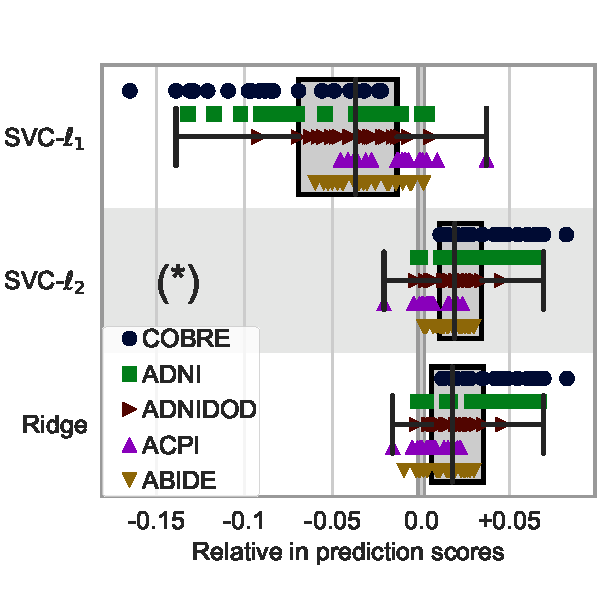
\includegraphics[width=0.8\linewidth]{figures/impact_plot_classifier.pdf}%
    }%
    \caption[choice of classifier]{\textbf{The impact of classifier
            choices in functional connectivity prediction pipeline over
            diverse tasks}:
            The figure shows the relative change to mean in prediction scores
            (AUC) over all the classifiers SVC-$\ell{_1}$, SVC-$\ell{_2}$,
            Ridge. Each boxplot depicts the prediction
            impact of each classifier grouped together for all datasets
            (COBRE, ADNI, ADNIDOD, ACPI, ABIDE) whereas each data point on top
            of each boxplot is a split of impact over each dataset.
            From the baseline=$0.0$, $\ell{_2}$ regularized choices such as
            SVC-$\ell{_2}$ and Ridge has
            shown relatively positive impact in prediction, significant
            across datasets. SVC-$\ell_{1}$ choice has shown negative impact in
            prediction across all datasets. For each choice, the prediction pipeline
            was ran in cross-validation framework with $n=100$ random splits
            and shuffled with $75\%$ training set and $25\%$ test set.
            } 
\label{fig:impact_classifier}
\end{figure}

\subsection{Choice of connectivity parameterization}
In \autoref{fig:impact_connectivity}, we show the relative impact of
the measure of covariance matrix/connectome method made on the classification
of diverse tasks from multi rs-fMRI datasets. We took the relatively mean over
all the connectivity parameterization methods (Full correlation, Partial
correlation, Tangent space parameterization) while demeaned the effect of
variance from remaining steps in the pipeline such as Brain ROIs and Linear
Classifiers.

From \autoref{fig:impact_connectivity}, we summarize that connectomes built
with tangent space parameterization outperformed other standard methods
such as full correlations and partial correlations.
Tangent space parameterization method has shown significantly positive impact
and consistent in finding the covariances across pair of brain ROIs, able
to use in discrimination across diverse tasks. From
\autoref{fig:impact_connectivity}, it is also interesting to see comparisons
between full correlation and partial correlation methods. Full correlation
has made an positive prediction impact on ADNI dataset to discriminate
between Alzheimer's disease (AD) and Mild Cognitive Impairment (MCI). Partial
correlation performed well in discriminating Marijuana users and Non-marijuana
users. Between full correlation and partial correlation, only predicting few
tasks has high impact where tangent space parameterization has significant
impact across diverse targets.

These results suggest that probabilistic approach leads to finding good
selection of connectivity features across brain regions to compare them across
subjects.


\begin{figure}
    \centerline{%
    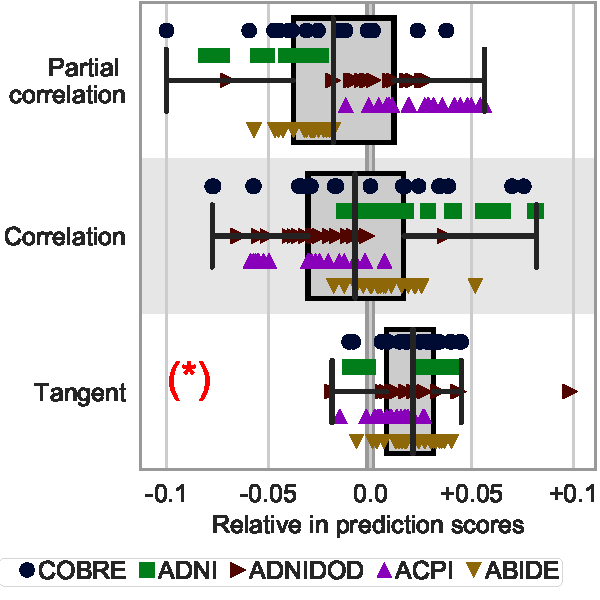
\includegraphics[width=0.8\linewidth]{figures/impact_plot_measure.pdf}%
    }%
    \caption[choice of connectome]{\textbf{The impact of connectivity
            parameterization methods in functional connectivity prediction
            pipeline over diverse tasks}:
            Boxplot (gray) ($x-axis$) is a relatively change in prediction scores
            (AUC) over all the connectivity methods - Full correlation, Partial
            correlation and Tangent space parameterization. Each boxplot
            depicts the prediction impact of each connectivity method grouped
            together for all datasets. Each data
            point on top of each boxplot shows the impact separately
            over each dataset (COBRE, ADNI, ADNIDOD, ACPI, ABIDE). Full and Partial
            correlation based connectivity performed less, showed
            large variations and minimal impact on predicting diverse tasks.
            While prediction using tangent space based connectivity
            parameterization has showed good impact and consistent where
            data points are falling almost in the positive range from
            baseline=$0.0$. For each choice, the prediction pipeline
            was ran in cross-validation framework with $n=100$ random splits
            and shuffled with $75\%$ training set and $25\%$ test set.
\label{fig:impact_connectivity}}
\end{figure}

\subsection{Choice of brain atlases}
To understand better the choice of brain atlas in prediction pipeline,
we first systematically compared the atlases composed of brain regions and
networks across enormous learning dimensions and
made an empirical choice of dimension on each atlas as outlined in
\autoref{fig:effect_size_in_regions} and \autoref{fig:effect_size_in_networks}.
Second, we adapted this comparison to study the relative impact of each
brain atlas made in pipeline prediction over diverse tasks as
outlined in \autoref{fig:impact_atlas}. Brain atlases have made a huge
impact in the prediction pipeline and each atlas has showed its significant
impact in predicting diverse tasks across all multi rs-fMRI datasets.
Data-driven atlases such as Ward, K-Kmeans, GroupICA and Online Dictionary
Learning had made a significant impact in predicting on COBRE and ADNI
datasets. While pre-defined anatomical atlases such as AAL and Harvard Oxford
have made less impact in predicting diverse tasks. Harvard Oxford is only
performing good on ACPI datasets. Out of all atlases, Online dictionary
learning had showed good positive impact where the relative scores across
diverse tasks are of positive values except in ADNIDOD.

\subsubsection{Choice of dimensionality with Brain regions}
In \autoref{fig:effect_size_in_regions}, we show the impact of the
learning dimensionality in brain atlases composed of regions
made on prediction scores. The
data-driven atlas extraction methods such as GroupICA (ICA), Online Dictionary
Learning (DictLearn), KMeans with enormous dimensions varied in ${40, 60,
80, 100, 120, 150, 200, 300}$, and a pre-defined functional atlas BASC built with
dimensionality varied in ${36, 64, 122, 197, 325, 444}$ are used for
comparisons to make an optimal choice of dimension for each method. From
\autoref{fig:effect_size_in_regions}, we chose optimal choice of
learning dimensionality with GroupICA as $80$, Online Dictionary Learning as
$60$, KMeans as $100$, BASC as $122$. We made the choice of learning
dimensionality which made high positive impact from the baseline=$0.0$ for
all multi rs-fMRI datasets - COBRE, ADNI, ADNIDOD, ACPI, ABIDE. We did not
study the already imposed spatially constrained Ward method in brain atlases
comparisons composed of regions. 

The choices of dimensionality learned for each atlas are further
used in comparing
for optimal choice between brain regions and brain networks as outlined in
\autoref{fig:regions_vs_nonregions} to study the comparisons of choices of
brain atlases.

\begin{figure}
    \centerline{%
    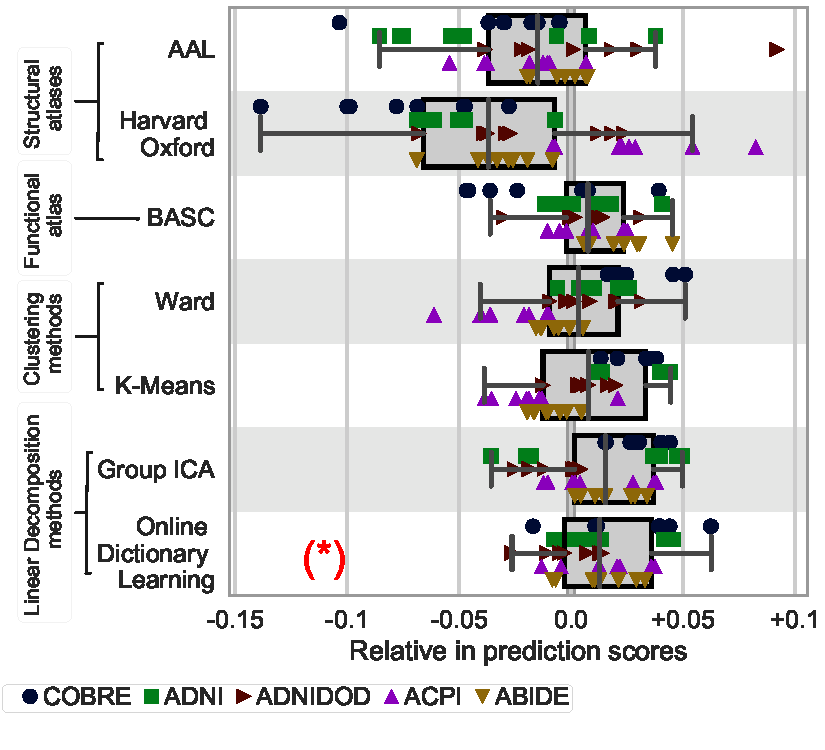
\includegraphics[width=\linewidth]{figures/impact_plot_atlas.pdf}%
    }%
    \caption[choice of atlas]{\textbf{The impact of brain atlases in
            functional connectivity prediction pipeline over diverse tasks}:
            Boxplot (gray) depicts the relatively change in prediction
            scores response in AUC ($x-axis$) over all the atlas choices on
            ($y-axis$) - AAL, Harvard Oxford, BASC, Ward, K-Means, Group ICA,
            Online Dictionary Learning grouped for all the multi rs-fMRI
            datasets. While each data point on top of each boxplot outlines
            the prediction impact separately for each dataset - COBRE (black),
            ADNI (green), ADNIDOD (dark red), ACPI (pink), ABIDE (brown).
            Learning atlases on the brain data had showed positive prediction
            impact significant over predicting diverse tasks, in particular,
            Online Dictionary Learning. The impact of using pre-defined
            anatomical atlases - AAL and Harvard Oxford is significantly less
            and has huge variance in the prediction of diverse tasks (highly
            dependant on the phenotype). The comparisons in this figure
            are made on particular choice of dimension chosen for each
            data-driven learning atlas: such as Ward of $120$ brain
            parcellations, K-Means of $100$ brain parcellations, Group ICA of
            $80$ brain networks and splitted into regions, Online Dictionary
            Learning of $60$ brain networks splitted into regions. We also
            pick dimension of one functional pre-defined atlas: BASC of $122$
            brain networks split into regions. These choices are made after
            systematic exploration across all dimensions used
            in the experiments to build the brain atlases for prediction. As
            showed in \autoref{fig:effect_size_in_regions} and
            \autoref{fig:effect_size_in_networks}, where choices on dimensions
            are made between regions or networks/parcellations. In
            \autoref{fig:regions_vs_nonregions}, where choice is made between
            regions or without regions. For all comparisons, the prediction
            pipeline was ran in cross-validation framework with $n=100$
            random splits and shuffled with $75\%$ training set and $25\%$
            test set.
    \label{fig:impact_atlas}}
\end{figure}


\begin{figure}
    \centerline{%
	\includegraphics[width=1.1\linewidth]{figures/dot_plot_n_regions_suppressed_background.pdf}%
    }%
    \caption[]{\textbf{Impact of dimensionality in learning the prediction with atlas of
            brain regions}: For each atlas - ICA, DictLearn, KMeans, BASC),
            violinplot (gray) depicts the relatively mean change in prediction
            scores response in AUC ($y-axis$) over all the dimensionalities
            ($x-axis$). On top of each violinplot are the error bars with
            $95\%$ confidence interval across all datasets - COBRE (black),
            ADNI (green), ADNIDOD (dark red), ACPI (pink), ABIDE (brown).
            The optimal dimensionality (vertical red arrow) with
            ICA is $80$, DictLearn is $60$,
            KMeans is $100$ and BASC is $122$ which has showed significantly
            positive impact (above baseline=$0.0$) across all datasets. We
            reduce the effect of variance by keeping the prediction scores
            from the pipeline only to tangent space parameterization and
            SVC-$\ell{_2}$ classifier. The pipeline prediction was ran in
            cross-validation framework with $n=100$ random splits shuffled with
            $75\%$ training set and $25\%$ test set.}
    %
    \label{fig:effect_size_in_regions}
\end{figure}

\subsubsection{Choice of dimensionality with Brain networks or parcellations}
%
In \autoref{fig:effect_size_in_networks}, the
atlas extraction methods such as GroupICA (ICA), Online Dictionary
Learning (DictLearn), KMeans and Ward with enormous dimensions varied in ${40, 60,
80, 100, 120, 150, 200, 300}$, and a pre-defined functional atlas BASC built with
dimensionality varied in ${36, 64, 122, 197, 325, 444}$ are used for
comparisons to make an optimal choice of dimension for each method (without
regions). From
\autoref{fig:effect_size_in_networks}, we chose optimal choice of
learning dimensionality with GroupICA as $80$, Online Dictionary Learning as
$60$, KMeans as $100$, Ward as $120$ and BASC as $122$. We made an empirical
choice of learning dimensionality by choosing the atlases which made high
positive impact
for all multi rs-fMRI datasets - COBRE, ADNI, ADNIDOD, ACPI, ABIDE. If any of the
both choice in each atlas have made an equal impact, we took the least
probable dimensionality as an optimal choice.
The choices of dimensionality learned for each atlas are further
used in comparing
for optimal choice between brain regions and brain networks as outlined in
\autoref{fig:regions_vs_nonregions} to study the comparisons of choices of
brain atlases.
\begin{figure}
    \centerline{%
	\includegraphics[width=1.1\linewidth]{figures/dot_plot_parcellations_suppressed_background.pdf}%
    }%
    \caption[]{\textbf{Impact of dimensionality in learning the prediction
            with atlas of brain networks/parcellations}
            For each atlas composed of networks (ICA, DictLearn, BASC)
             and parcellations (KMeans and Ward), violinplot (gray)
             depicts the relatively mean change in prediction
            scores response in AUC ($y-axis$) over all the dimensionalities
            ($x-axis$). On top of each violinplot are the error bars with
            $95\%$ confidence interval across all datasets - COBRE (black),
            ADNI (green), ADNIDOD (dark red), ACPI (pink), ABIDE (brown).
            The optimal dimensionality (vertical red arrow) with
            ICA is $80$, DictLearn is $60$,
            KMeans is $100$ , Ward is $120$ and BASC is $122$ which has
            showed significantly
            positive impact (above baseline=$0.0$) across all datasets. We
            reduce the effect of variance by keeping the prediction scores
            from the pipeline only to tangent space parameterization and
            SVC-$\ell{_2}$ classifier. The pipeline prediction was ran in
            cross-validation framework with $n=100$ random splits shuffled with
            $75\%$ training set and $25\%$ test set.}
    %
    \label{fig:effect_size_in_networks}
\end{figure}

\subsubsection{Which is better: Brain atlases with regions or without regions}
Given the outlined choices of optimal dimensionality in brain atlases composed
of regions and networks as shown in \autoref{fig:effect_size_in_regions}
and \autoref{fig:effect_size_in_networks}, we compare now to study which has
better impact in prediction. Prediction using atlases composed of regions or
networks. As shown in
\autoref{fig:regions_vs_nonregions}, atlases with GroupICA or ICA, predicting
using regions is better rather than using only networks. Whereas for
Dictionary Learning, prediction using regions is better and same even with
BASC atlases. Interesting, to see that BASC which is a pre-defined atlase
built on unseen resting state functional datasets is better with regions
rather than only networks. While we see the opposite with KMeans based atlas
prediction. With KMeans, using parcellations without regions or
inter-hemispheric separation is better for prediction tasks of resting state
fMRI.

%\begin{table}[tb]
%\footnotesize%
%\small
%\rowcolors{2}{gray!15}{white}%
%\begin{tabularx}{\linewidth}{p{1.0cm}|l|l|l|l}
%    \textbf{Brain atlas} & \textbf{Connectivity}
%    & \textbf{Classifier} & \textbf{Regions} & \textbf{Dimensions} \\
%    %\hline
%    DictLearn & Tangent Embedding & SVC-$\ell{_2}$ & Yes & 60 \\
%    %\bottomrule
%\end{tabularx}
%\end{table}

\begin{figure}
    \centerline{%
	\includegraphics[width=1.\linewidth]{figures/regions_networks_difference_distribution.pdf}%
    }%
    \caption[regions vs non regions]{\textbf{Which is better for prediction:
            Brain regions or Brain networks}
        For each atlas (ICA, DictLearn, KMeans and BASC), we show here the
        best setting for prediction by measuring its impact on prediction
        accuracy for each dataset.

        Each data point is a measure of impact on prediction accuracy. For
        each atlas, data point in unique color is a score obtained by averaging
        raw prediction scores grouped by three classifiers, three measures.
        Each unique color is referred to each of four datasets used to test
        the prediction. 

        We then compare these data points using violin plots with or without
        region extraction. On x-axis is the impact on prediction and on y-axis
        is to differentiate between region extraction and no region extraction.

        From the observations, ICA atlas based prediction has better impact
        by extracting regions on the networks which is quite similarly
        observed with Online Dictionary Learning and BASC. But, KMeans has
        better impact when predicted using without region extraction meaning
        that parcellations based atlas.
    %
    \label{fig:regions_vs_nonregions}
    }
\end{figure}


\begin{figure}
    \centerline{%
	\includegraphics[width=0.5\paperwidth]{figures/brainrois.pdf}%
    }%
    \caption{\textbf{Brain regions/parcellations using ICA, DictLearn, KMeans,
        Ward}
    %
    %
    \label{fig:brain_rois}
    }
\end{figure}
\paragraph{Choice of brain atlas}

\section{Discussion:}

In this section, we talk about the right trends and recommendations which
should be made at each step in the functional connectivity prediction
pipeline.

\section{Conclusion:}

\subsection*{Acknowledgments}

Funded by NiConnect project (ANR-11-BINF-0004\_NiConnect) and CATI.

% references section


\section{Supplementary material}
%\bibliographystyle{elsarticle-num-names}
\bibliography{biblio}

\end{document}

